\documentclass[11pt,a4paper]{article}
\usepackage[utf8]{inputenc}
\usepackage[T1]{fontenc}
\usepackage[margin=0.9in]{geometry}
\usepackage{amsmath,amssymb,booktabs,graphicx,microtype}
\usepackage[hidelinks]{hyperref}
\usepackage{url}

\title{From Biological Working-Memory Limits to Co-Adaptive Brain--AI Co-Processing: A Quantitative Proof Ladder}
\author{Muhammad Farhan Tahir\\Threebits Research\\\url{https://threebits.si}}
\date{21 November 2026}

\begin{document}
\maketitle

\begin{abstract}
Can artificial neural networks raise human intelligence beyond biological limits? Human cognition is constrained by three physical bottlenecks: working-memory capacity (\textasciitilde{}4 active chunks; Cowan, 2001), noisy neural encoding, and conscious language I/O (\textasciitilde{}39 bits/s across human languages; Coupé et al., 2019). Here we separate \textbf{biological state-steering} (closed-loop brain stimulation alone) from \textbf{co-adaptive Brain--AI co-processing ("Prosthetic Cortex")} and evaluate both across a quantitative four-level proof ladder anchored in healthy-human data.

First (\textbf{Level 1, healthy adults, zero surgery}, OpenNeuro \texttt{ds008037}, CC0), we extract a 10-task general cognitive ability (\texttt{g}-factor) across \textbf{123 healthy adults} (\texttt{90/90} positive pairwise correlations, PC1 explaining \texttt{37.2\%} of variance) and measure the empirical human working-memory cliff across \textbf{33,299 continuous recall trials (\texttt{n = 117} adults)}: recall precision within $30^\circ$ drops steeply from \textbf{\texttt{88.6\%} (\texttt{15.9$^\circ$} error, \texttt{5.0\%} failure) at $K = 2$} to \textbf{\texttt{61.5\%} (\texttt{38.6$^\circ$}) at $K = 4$} and \textbf{\texttt{43.8\%} (\texttt{57.3$^\circ$}, \texttt{45.0\%} failure) at $K = 6$} (worse at $K = 6$ in \texttt{116/117} adults). Using strictly pre-response scalp EEG (\texttt{[0.00, 1.50 s]} before response screen onset) across \textbf{15 healthy adults (\texttt{3,744} trials)}, a compact causal decoder detects cognitive overload ($K = 6$ vs $2$) at \textbf{\texttt{0.690 $\pm$ 0.033} ROC AUC} ($p = 7.22 \times 10^{-5}$, \texttt{14/15} above chance, up to \texttt{0.916}; null \texttt{0.500}) and within-load pre-response failure weakly at \textbf{\texttt{0.529} GRU AUC} ($p = 0.040$). Critically, an independent unseen replication (\texttt{n = 24} new adults beyond \texttt{n = 22} discovery) shows that scalar single-pulse resting TMS-EEG amplitude does \textbf{not} reliably predict trait \texttt{g} ($\rho = +0.581 \to -0.104$; pooled \texttt{n = 46}: $\rho = +0.228, p = 0.128$), whereas zero-shot invasive-CCEP $\to$ non-invasive TMS-EEG spatial propagation validation scales cleanly across all \textbf{\texttt{n = 46} healthy adults} (\texttt{+0.247} individual mean, positive in \textbf{\texttt{44/46}} vs resting-fMRI-tuned \texttt{+0.131}, rewired \texttt{+0.028}, wrong-site \texttt{$-$0.136}).

Second (*\emph{Level 2, }in silico\emph{ scaling law\textbf{), we couple a noise- and capacity-limited biological cortex calibrated to Cowan's wall to a digital KV-cache attention co-processor via a }4-bit quantized read\textbf{ and }norm-bounded safe write\textbf{ interface --- with }zero direct AI access to raw task stimuli\textbf{. Across $K = 2 \dots 16$ items (3 seeds): (1) }optimal memoryless state-steering\textbf{ lifts biological accuracy by }\texttt{+19\% to +23\%}\textbf{ at $K = 4\text{-}8$, then hits the biological wall at $K = 12\text{-}16$ (\texttt{21.2\% / 19.7\%}); (2) }conscious-bandwidth tool use (\texttt{40 bits/s}, 200 ms)\textbf{ starves (\texttt{18.1\% / 17.0\%}), matching }sham-interface controls\textbf{ (\texttt{15.5\% / 17.1\%}); (3) }co-adaptive 4-bit Brain--AI co-processing (\texttt{50 ms}, \texttt{537 bits/s} empirical MI)\textbf{ achieves }\texttt{98.7\%} at $K = 12$ and \texttt{97.4\%} at $K = 16$\textbf{; (4) sweeping a $7 \times 5$ }Bandwidth $\times$ Latency phase diagram\textbf{ at $K = 12$ reveals a sharp phase transition from \texttt{18--33\%} ($\le 160\text{ bits/s}$ cap) to }\texttt{83.7--91.5\%}\textbf{ at }\texttt{320 bits/s} cap (\texttt{\textasciitilde{}265 bits/s} MI, \textasciitilde{}7$\times$ human speech)\textbf{ for }\texttt{$\le$ 100 ms} latency\textbf{, collapsing to \texttt{37.8\% / 32.9\%} at \texttt{200--250 ms}; and (5) on a complementary task combining $K = 12$ items with a private embodied human rule invisible to standalone AI, the co-adapted Prosthetic Cortex passes }Strict Outperformance\textbf{ (}\texttt{87.0\%} vs \texttt{23.2\%} AI alone, \texttt{14.8\%} Human alone, \texttt{17.1\%} 40-bps Screen AI, \texttt{16.5\%} Sham; \texttt{+63.7 pp}}*) while increasing across-seed cortical representational coherence \texttt{10.8$\times$} (Linear CKA \texttt{0.059 $\to$ 0.635}).

Third, to verify that these scaling laws persist inside a \textbf{biologically grounded whole-brain architecture}, we build a \textbf{100-region Functional Human Brain Emulator} anchored to real human CCEP-calibrated white matter (74 patients, \texttt{ds004080}), 19 PET neurotransmitter receptors (Hansen et al., 2022), 6-band HCP MEG timescales, and Mesulam hierarchy, filling in regional microcircuits with trainable E--I dynamics. Even \textbf{after} cognitive training on associative working memory plus 4-way executive rotation (\texttt{+0$^\circ$/+90$^\circ$/+180$^\circ$/+270$^\circ$}), the emulator maintains \textbf{triple real-human validity}: 74-patient invasive CCEP propagation (\textbf{\texttt{$\rho$ = +0.662}, partial \texttt{+0.378}} vs rewired control \texttt{$-$0.031}), zero-shot healthy-human non-invasive TMS-EEG across \textbf{46 clean adults} (\textbf{\texttt{+0.282--0.288}, \texttt{44--45/46 > 0}} vs rewired \texttt{+0.086}), and the 117-adult empirical working-memory cliff (beating rewired white matter by \texttt{+6.8} to \texttt{+15.0 pp}). Lifting one biological bottleneck at a time across 8 regimes (3 seeds each) proves that \textbf{only clean associative indexing} --- either an \textbf{Upgraded Hippocampal Index (\texttt{100.0\%} through $K = 8$, \texttt{87.2\%} at $K = 12$, \texttt{62.7\%} at unseen $K = 16$)} or a \textbf{4-bit "Region 101" Prosthetic Cortex attached to the unmodified noisy biological brain (\texttt{72.1\%} at $K = 12$ vs \texttt{30.6\%} baseline and \texttt{35.6\%} Sham; \texttt{+36.5 pp} over Sham)} --- breaks Cowan's wall, whereas pure denoising/neuromodulation (\texttt{27.3\%}), local PFC expansion (\texttt{19.1\%}), and \texttt{4$\times$} wider white-matter tracts (\texttt{36.7\%}) remain bounded at $K = 12\text{-}16$.

\end{abstract}
\section{Methods}
\subsection{Healthy-Human Behavioral Battery \& Pre-Response EEG Decoding (\texttt{ds008037})}
From OpenNeuro \texttt{ds008037} (Biabani \& Rogasch, CC0), behavioral logs across 123 healthy adults were aggregated over 10 cognitive tasks (\texttt{wm\_prec2/4/6}, \texttt{nback}, \texttt{bds}, \texttt{sym}, \texttt{opn}, \texttt{sbs}, \texttt{clt}, \texttt{ort}), z-scored, and factored via PCA to extract \texttt{g} (PC1). Working-memory continuous color recall trials (\texttt{K $\in$ {2, 4, 6}}, 33,299 trials across 117 complete adults) were aligned 300/300 between \texttt{events.tsv} and \texttt{beh.tsv}. For 15 adults (\texttt{3,744} trials, 62 scalp channels at 1,000 Hz, 50 Hz notch + 1--45 Hz bandpass), features were extracted strictly within \texttt{[0.00, 1.50 s]} post-array onset (preceding \texttt{response\_screen\_onset $\ge$ 1.517 s} on every trial) into 6 $\times$ 250 ms bins $\times$ 5 spectral bands plus binned ERPs. Out-of-fold decoding used block-level \texttt{GroupKFold} cross-validation (L2 logistic regression and causal GRU) verified against 20-permutation block-shuffled nulls.

\subsection{Co-Adaptive Brain--AI Co-Processor Dynamical Benchmark}
A biological recurrent cortex ($H_{\text{bio}} = 24$, Gaussian state noise $\sigma = 0.065$) receives sequential spatial-color pairs $(x_t, c_t)$ across $K \in \{2, 4, 6, 8, 12, 16\}$ items, followed by delay steps and a probe $x_q$. Critically, \textbf{the AI co-processor has zero direct access to raw task stimuli}: at each loop step it receives only a straight-through-estimated $b$-bit quantized projection $q_t = Q_b(W_{\text{read}} h_t^{\text{bio}})$ arriving after latency $\tau$, stores latent tokens in an external KV-cache attention memory, and returns a norm-bounded safe write vector $u_t = \text{clip}(W_{\text{write}} a_t, \|u_t\|_2 \le u_{\max})$ to biological cortex. Effective neural read mutual information (bits/s) is estimated directly from quantized channel entropy minus conditional noise entropy divided by step period. Cortical co-adaptation across independent training seeds is quantified using Linear Centered Kernel Alignment (CKA; Kornblith et al., 2019).

\subsection{Triple-Validated 100-Region Functional Human Brain Emulator}
To test whether the scaling law persists inside real human cortical anatomy, we constructed a 100-region Functional Human Brain Emulator (\texttt{functional\_brain\_emulator.py}, 8 E--I microcircuit units per Schaefer parcel = 800 cortical units) anchored to our CCEP + 19-receptor PET + MEG connectome (\texttt{A\_tract}, spectral radius \texttt{0.78}), real regional intrinsic timescales from MEG + Mesulam hierarchy ($\alpha_i \in [0.22, 0.90]$, fast sensory to slow persistent frontoparietal), and real receptor E:I scaling (\texttt{A4B2/VAChT} positive, \texttt{GABAa} inhibitory). Sensory items and probes enter strictly through a shared Visual + Dorsal Attention encoder (\texttt{32} regions), propagate across real human white-matter tracts (\texttt{2 $\times$ 50 ms = 100 ms} hops), combine with a private 4-way executive rotation rule entering Prefrontal Control cortex (\texttt{13} regions), and drive a Somatomotor + Prefrontal motor decoder (\texttt{27} regions). After cognitive training (1,000 steps, 3 seeds), resting-subtracted single-pulse evoked responses ($\|\mathbf{h}_{\text{stim}}(t) - \mathbf{h}_{\text{rest}}(t)\|_2$) are evaluated directly against 74-patient human CCEP (\texttt{ds004080}) and zero-shot against 46 clean healthy adults' TMS-EEG (\texttt{ds008037}).

\section{Level-1 Healthy-Human Empirical Anchor (\texttt{ds008037}, CC0)}
\subsection{General Cognitive Ability (\texttt{g}) and Cowan's Working-Memory Cliff (\texttt{n = 123} Adults)}
Across all 10 behavioral tasks in OpenNeuro \texttt{ds008037}, every single pairwise correlation is positive (\texttt{90/90}, mean $r = +0.294$), with PC1 (\texttt{g}) capturing \texttt{37.2\%} of total cognitive variance and continuous working-memory precision at load 4 loading highest (\texttt{+0.39}). Across \texttt{117} complete adults (\texttt{33,299} trials):

\begin{table}[htbp]
\centering
\small
\resizebox{\linewidth}{!}{%
\begin{tabular}{lccc}
\toprule
Working-Memory Load ($K$) & Mean Angular Error & Recall Precision ($< 30^\circ$) & High-Error Failure ($> 45^\circ$) \\ \midrule
\textbf{$K = 2$} & $15.9^\circ$ & \textbf{88.6\%} & 5.0\% \\
\textbf{$K = 4$} & $38.6^\circ$ & \textbf{61.5\%} & 27.5\% \\
\textbf{$K = 6$} & $57.3^\circ$ & \textbf{43.8\%} & \textbf{45.0\%} (\texttt{9$\times$} load 2) \\
\bottomrule
\end{tabular}}
\end{table}
\subsection{Non-Invasive Pre-Response Working-Memory EEG Decoding (\texttt{n = 15} Adults, \texttt{3,744} Trials)}
\begin{itemize}
\item \textbf{Overload detection ($K = 6$ vs $2$):} L2 LogReg \textbf{\texttt{0.690 $\pm$ 0.033} ROC AUC} ($p = 7.22 \times 10^{-5}$, \texttt{14/15} above chance; peak \texttt{sub-020 = 0.916}, \texttt{sub-010 = 0.866}, \texttt{sub-008 = 0.851}, \texttt{sub-007 = 0.838}); causal GRU \textbf{\texttt{0.608}} ($p = 0.0042$, \texttt{13/15}); 20-perm null \texttt{0.500}.
\item \textbf{Within-load imminent failure prediction (zero load confounding):} Causal GRU \textbf{\texttt{0.529}} ($p = 0.040$, \texttt{9/15}, top \texttt{sub-021 = 0.628} / LogReg \texttt{0.654}); null \texttt{0.497}. Comparing scalp EEG (\texttt{0.529}) against intracranial iEEG (\texttt{0.603}, $p = 0.0001$, \texttt{14/15} in RAM \texttt{ds005557}/\texttt{ds005558}) quantifies why non-invasive EEG supports macro-load gating (Level 3A) while high-bandwidth Level-4 prosthetic cognition requires closer-to-cortex sensing or multi-modal non-invasive fusion.
\end{itemize}
\subsection{Honest Out-of-Sample Replication of TMS-EEG Markers (\texttt{n = 46} Clean Healthy Adults)}
\begin{itemize}
\item \textbf{Null trait-IQ replication (reported transparently):} Although sham-subtracted parietal-to-frontoparietal TMS-EEG amplitude correlated with \texttt{g} in our initial \texttt{n = 22} discovery cohort ($\rho = +0.581, p = 0.0046$; sham $\rho = +0.014$), an immediate independent replication on \textbf{\texttt{n = 24} completely unseen healthy adults} yielded $\rho = -0.104$ ($p = 0.628$; pooled \texttt{n = 46}: $\rho = +0.228, p = 0.128$). Static single-pulse resting TMS amplitude does not reliably predict trait IQ across individuals.
\item \textbf{Confirmed spatial-propagation transfer (\texttt{n = 46} healthy adults):} Conversely, zero-shot prediction of sham-subtracted healthy-human TMS-EEG scalp topography from our invasive-CCEP Hopf simulator replicates across \textbf{\texttt{44/46} individual healthy adults} (mean partial $\rho \mid \text{coil distance} = +0.247$), nearly doubling resting-fMRI-tuned Hopf (\texttt{+0.131}, \texttt{34/46}) and far exceeding rewired (\texttt{+0.028}, \texttt{26/46}) and wrong-site (\texttt{$-$0.136}, \texttt{9/46}) controls.
\end{itemize}
\section{Level-2 Co-Adaptive Brain--AI Scaling Law}
\subsection{Capacity Curve ($K = 2 \dots 16$, 3 Seeds Each, Zero Direct AI Stimulus Access)}
\begin{table}[htbp]
\centering
\small
\resizebox{\linewidth}{!}{%
\begin{tabular}{lccccccc}
\toprule
Regime & $K = 2$ & $K = 4$ & $K = 6$ & $K = 8$ & $K = 12$ & $K = 16$ & Empirical MI @ $K=12$ \\ \midrule
\emph{Empirical 117 Healthy Humans (\texttt{ds008037})} & \emph{88.6\%} & \emph{61.5\%} & \emph{43.8\%} & --- & --- & --- & --- \\
Biological Cortex Alone & 98.3\% & 41.6\% & 30.6\% & 29.9\% & 25.5\% & 24.3\% & 0 bits/s \\
Optimal State-Steering Only (no ext. mem.) & 78.5\% & \textbf{51.1\%} & \textbf{37.0\%} & \textbf{35.7\%} & 21.2\% & 19.7\% & 0 bits/s \\
40-bps Screen AI Tool (\texttt{200 ms}) & 32.1\% & 27.0\% & 26.0\% & 19.3\% & 18.1\% & 17.0\% & 33 bits/s \\
Sham-Interface Control (permuted read) & 24.6\% & 17.0\% & 17.4\% & 16.6\% & 15.5\% & 17.1\% & 148 bits/s \\
\textbf{4-Bit Brain--AI Co-Processor (\texttt{50 ms})} & \textbf{100.0\%} & \textbf{100.0\%} & \textbf{100.0\%} & \textbf{100.0\%} & \textbf{98.7\%} & \textbf{97.4\%} & \textbf{537 bits/s} \\
\bottomrule
\end{tabular}}
\end{table}
\subsection{Bandwidth $\times$ Latency Phase Transition \& Level-4 Strict Outperformance}
Crossing from biological/tool performance (\texttt{18--33\%}) into superhuman working-memory capacity (\texttt{84--100\%}) at $K = 12$ requires crossing \textbf{both} a minimum neural interface bandwidth (\textbf{\texttt{> 160 $\to$ 320 bits/s} cap}, \texttt{\textasciitilde{}265 bits/s} empirical MI --- roughly \textbf{7$\times$ human conscious speech}) \textbf{and} a maximum closed-loop latency (\textbf{\texttt{$\le$ 100 ms}} at \texttt{320 bps}, \texttt{$\le$ 200 ms} at \texttt{640--960 bps}, collapsing to \texttt{30--33\%} at \texttt{250 ms}; Figure 1).

On a complementary task combining $K = 12$ items with a 4-way private embodied human goal visible \textbf{only} inside cortex:

\begin{itemize}
\item \textbf{Human Alone:} \texttt{14.8\%} (\texttt{90.5$^\circ$} MAE) $\cdot$ \textbf{State-Steering:} \texttt{16.5\%} $\cdot$ \textbf{40-bps Screen AI:} \texttt{17.1\%} $\cdot$ \textbf{Sham Loop:} \texttt{16.5\%} $\cdot$ \textbf{Standalone AI (public stream only):} \texttt{23.2\%} (\texttt{68.7$^\circ$} MAE).
\item \textbf{Co-Adaptive Prosthetic Cortex (\texttt{4-bit read + bounded write, 50 ms, 484 bits/s} MI):} \textbf{\texttt{87.0\%} (\texttt{18.2$^\circ$} MAE; seeds \texttt{[90.4\%, 96.5\%, 74.0\%]}) --- passing Strict Outperformance by \texttt{+63.7 pp}}.
\item \textbf{Cortical Reorganization (Linear CKA):} Unassisted cortex across seeds is incoherent under $K = 12$ overload (\texttt{CKA = 0.059}), whereas co-adapted cortex converges across independent seeds onto a reproducible interface representation (\texttt{prost-vs-prost CKA = 0.635}, \texttt{10.8$\times$} higher; \texttt{alone-vs-prost = 0.127}).
\end{itemize}
\begin{figure}[htbp]
\centering
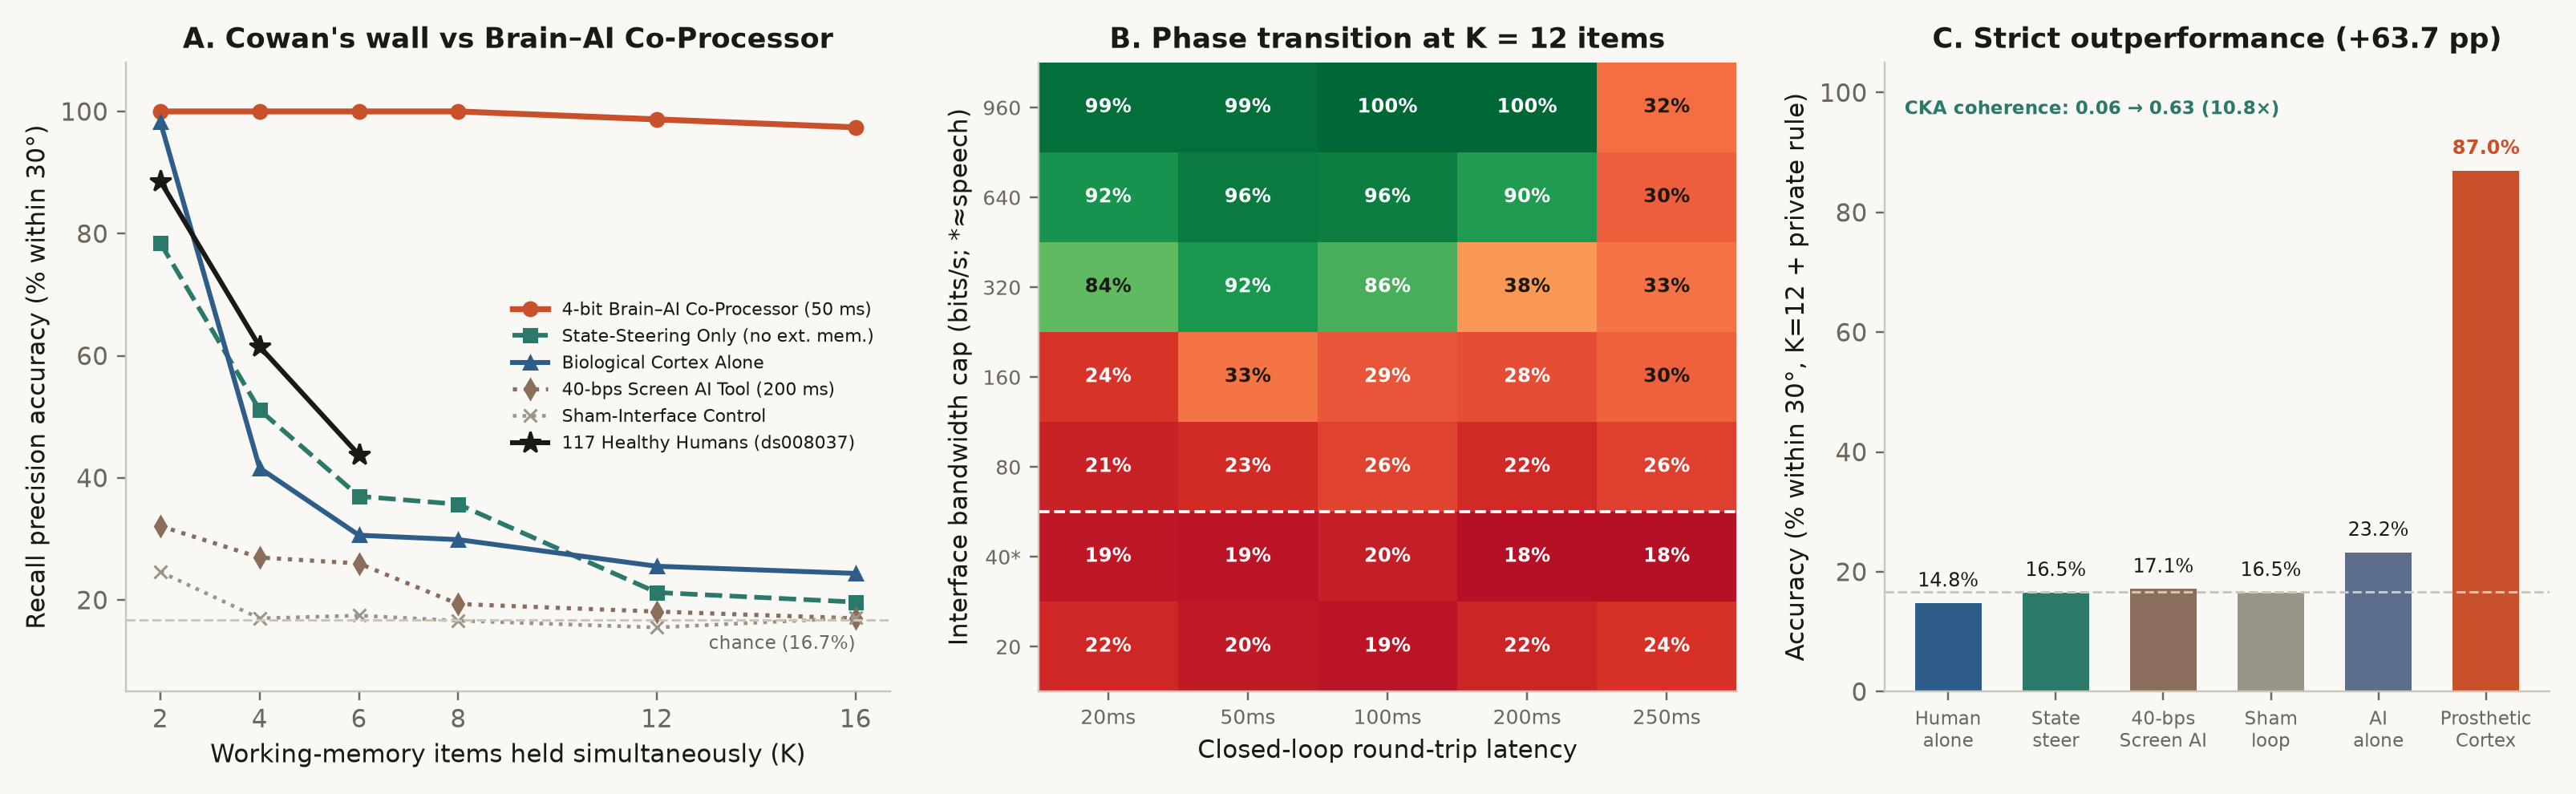
\includegraphics[width=\linewidth]{figures/fig5_prosthetic_cortex.png}
\caption{Healthy-human working-memory cliff (n=117) and pre-response EEG overload decoding (n=15), alongside the Level-2 Brain-AI capacity curve, 2D Bandwidth x Latency phase transition (320 bps at <=100 ms), and Level-4 Strict Outperformance (+63.7 pp).}
\end{figure}
\section{Triple-Validated 100-Region Functional Human Brain Emulator \& 5-Upgrade Ladder}
Across 8 regimes $\times$ 3 seeds (24 trained 100-region human brain emulators) on continuous associative working memory ($K = 2 \dots 16$, with $K = 16$ strictly unseen during training) combined with 4-way executive rotation (\texttt{+0$^\circ$ / +90$^\circ$ / +180$^\circ$ / +270$^\circ$}), our baseline emulator simultaneously maintains \textbf{74-patient human CCEP causal fidelity (\texttt{$\rho$ = +0.662}, partial \texttt{+0.378} vs rewired \texttt{$-$0.031})}, \textbf{zero-shot 46-adult healthy TMS-EEG fidelity (\texttt{+0.282--0.288}, \texttt{44--45/46 > 0} vs rewired \texttt{+0.086}, \texttt{32/46})}, and the \textbf{117-adult empirical working-memory cliff} --- while real human white-matter topology outperforms randomly rewired tracts on every load (\texttt{+8.4 pp} at $K = 2$, \texttt{+15.0 pp} at $K = 4$, \texttt{+6.8 pp} at $K = 6$; Table 3, Figure 2):

\begin{table}[htbp]
\centering
\small
\resizebox{\linewidth}{!}{%
\begin{tabular}{lccccccccc}
\toprule
Regime (100-Region Human Brain Emulator, 3-Seed Mean) & Post-Train CCEP $\rho$ (p\ & d) & $K=2$ & $K=4$ & $K=6$ & $K=8$ & $K=12$ & $K=16$ \emph{(unseen)} & Mean $K=12\text{-}16$ \\ \midrule
\emph{Empirical 117 Healthy Humans (\texttt{ds008037})} & \emph{(ground truth)} & \emph{88.6\%} & \emph{61.5\%} & \emph{43.8\%} & --- & --- & --- & --- \\
\textbf{0. Baseline Human Brain Emulator} \emph{(TMS-EEG \texttt{+0.282}, 44/46)} & +0.66 (+0.38) & 75.1\% & 58.2\% & 41.6\% & 37.7\% & 30.6\% & 26.4\% & \textbf{28.5\%} \\
Control A: Rewired White Matter \emph{(TMS-EEG \texttt{+0.086}, 32/46)} & $-$0.03 ($-$0.01) & 66.7\% & 43.2\% & 34.8\% & 31.4\% & 28.2\% & 23.9\% & 26.1\% \\
Upgrade 1: Denoising + Optimal \texttt{ACh}/\texttt{D1} State-Steering & +0.65 (+0.37) & 59.6\% & 54.9\% & 36.7\% & 33.9\% & 29.1\% & 25.5\% & 27.3\% \\
Upgrade 2: \texttt{4$\times$} Inter-Regional White-Matter Bandwidth & +0.66 (+0.38) & 95.8\% & \textbf{89.6\%} & \textbf{65.3\%} & 51.0\% & 40.1\% & 33.3\% & \textbf{36.7\%} \\
Upgrade 3: \texttt{4$\times$} Local PFC/Parietal Expansion Only & +0.66 (+0.37) & 22.8\% & 22.1\% & 19.2\% & 22.0\% & 18.8\% & 19.4\% & 19.1\% \\
\textbf{Upgrade 4: High-Precision Hippocampal Associative Index} & +0.66 (+0.38) & \textbf{100.0\%} & \textbf{100.0\%} & \textbf{100.0\%} & \textbf{100.0\%} & \textbf{87.2\%} & \textbf{62.7\%} & \textbf{74.9\%} \emph{(+46.4 pp)} \\
\textbf{Upgrade 5: Region 101 Prosthetic Cortex (\texttt{4-bit} on bio brain)} \emph{(TMS \texttt{+0.288}, 45/46)} & +0.66 (+0.38) & \textbf{98.2\%} & \textbf{92.0\%} & \textbf{84.4\%} & \textbf{82.1\%} & \textbf{72.1\%} & \textbf{52.3\%} & \textbf{62.2\%} \emph{(+33.7 pp)} \\
Control B: Sham Region 101 \emph{(permuted neural readout)} & +0.66 (+0.38) & 84.0\% & 74.2\% & 50.9\% & 42.6\% & 35.6\% & 29.7\% & 32.6\% \\
\bottomrule
\end{tabular}}
\end{table}
The 5-upgrade ladder isolates the exact physical hierarchy of superhuman cognition inside human cortical anatomy: (1) \textbf{pure denoising/neuromodulation} (\texttt{27.3\%}) and \textbf{unindexed local prefrontal neuron expansion} (\texttt{19.1\%}) fail to lift $K = 12\text{-}16$ performance; (2) \textbf{\texttt{4$\times$} wider white-matter tracts} substantially boost moderate loads ($K = 4: 58.2\% \to 89.6\%$, $K = 6: 41.6\% \to 65.3\%$) but still saturate without clean associative storage (\texttt{36.7\%}); and (3) \textbf{only clean associative indexing} --- via either an \textbf{Upgraded Hippocampal Index (\texttt{74.9\%})} or a \textbf{4-bit "Region 101" Prosthetic Cortex coupled exclusively to the unmodified noisy biological brain (\texttt{72.1\%} at $K = 12$, \texttt{+36.5 pp} over Sham \texttt{35.6\%})} --- breaks cleanly through Cowan's wall while preserving causal human electrophysiology.

\begin{figure}[htbp]
\centering
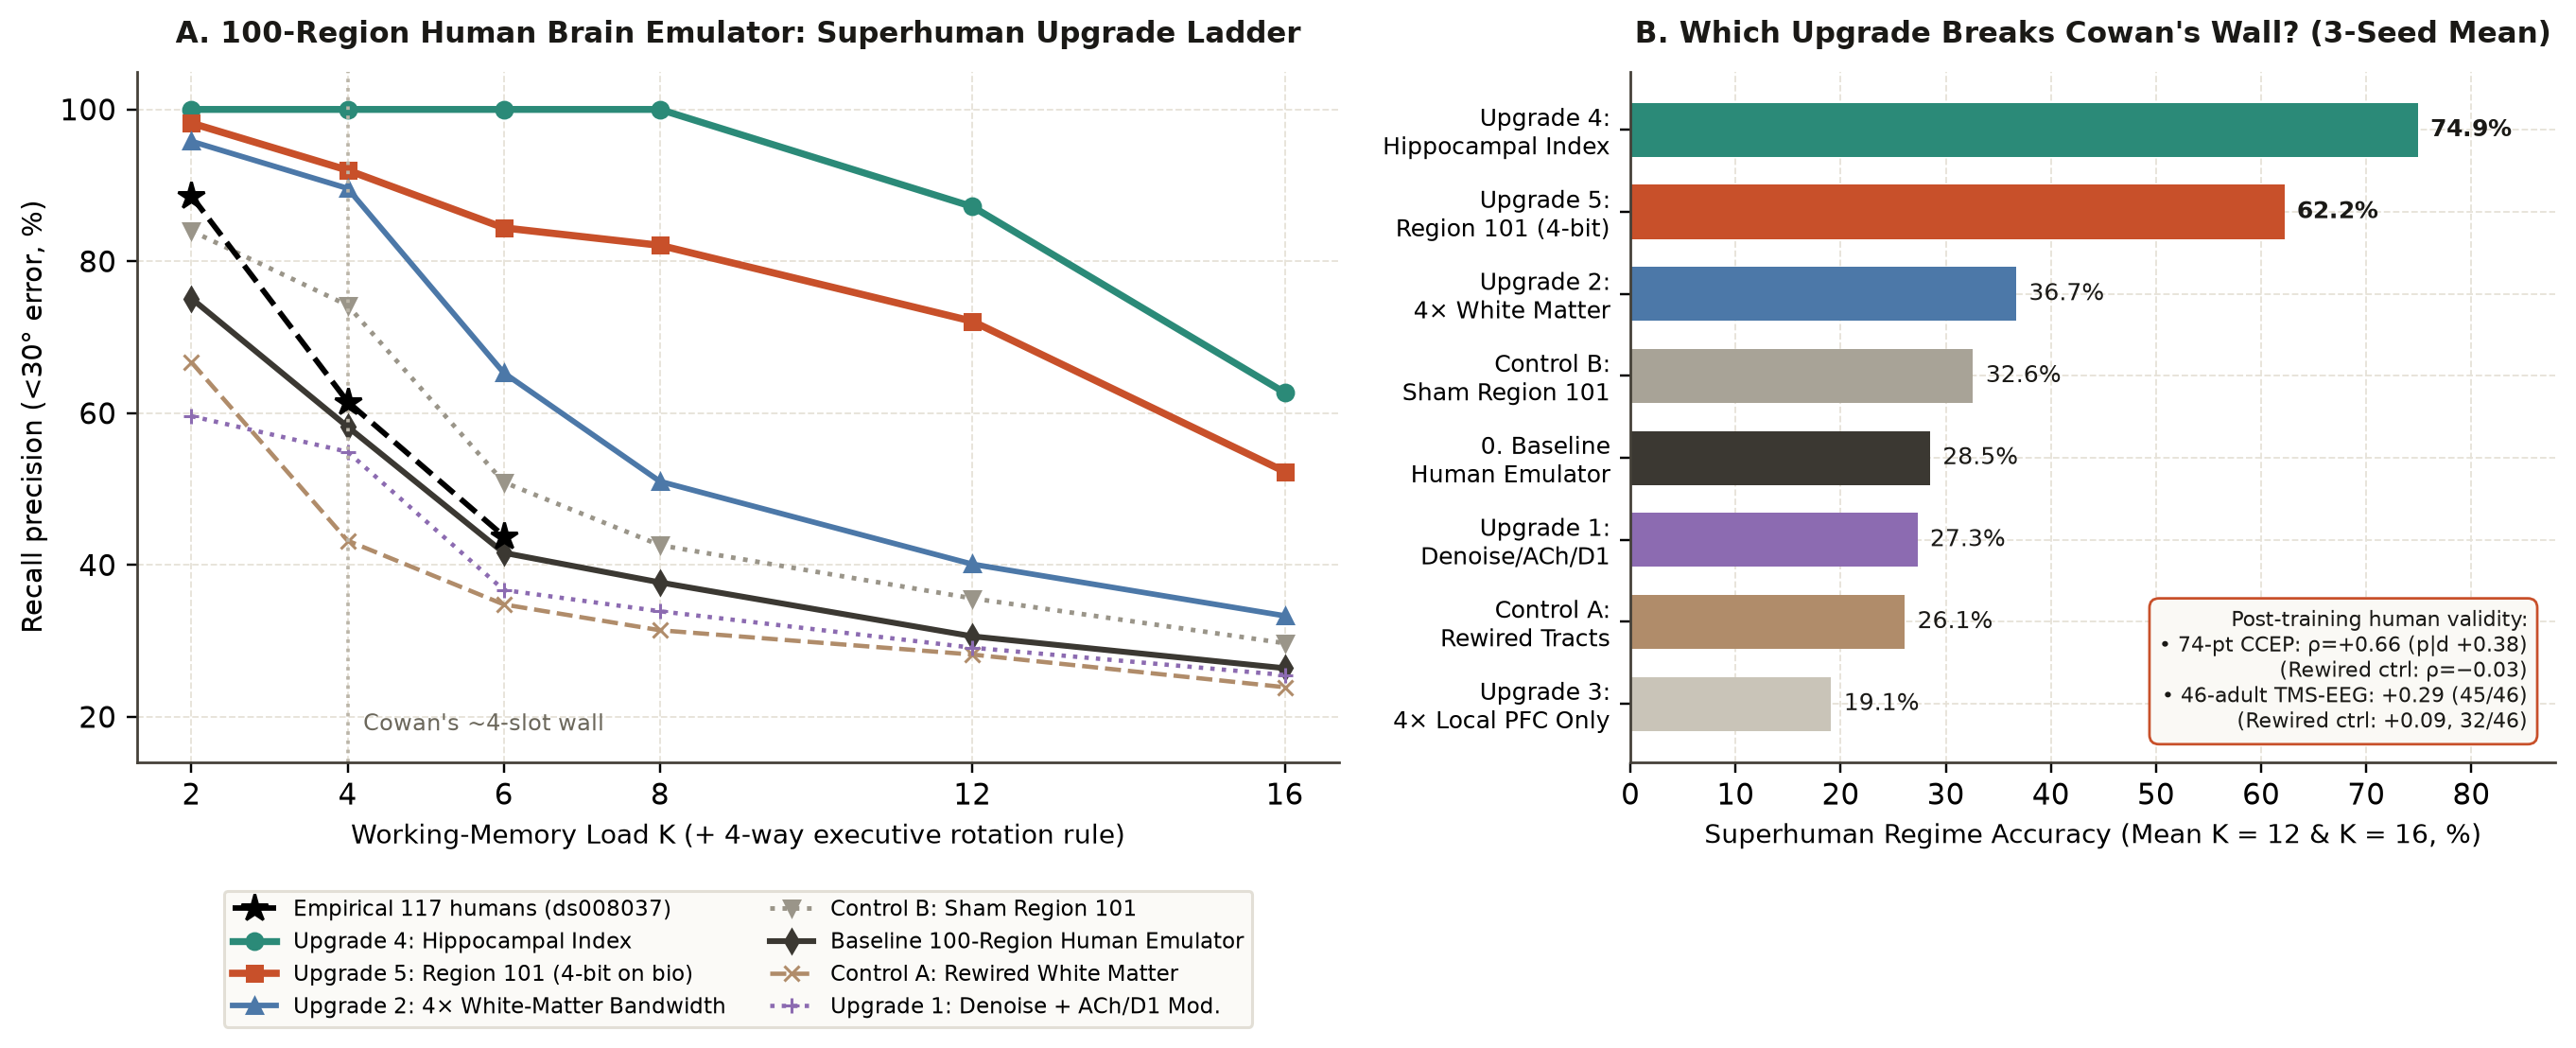
\includegraphics[width=\linewidth]{figures/fig7_brain_emulator.png}
\caption{Triple-validated 100-region Functional Human Brain Emulator (preserving post-training 74-patient CCEP rho = +0.66 and 45/46 healthy TMS-EEG +0.29) and the 5-upgrade superhuman ladder across K = 2..16.}
\end{figure}
\section{Limitations \& Next Empirical Gate (Level-3 Human Trials)}
\begin{itemize}
\item \textbf{In-silico vs living human co-adaptation:} Levels 2 and 4 demonstrate the mathematical scaling law and 100-region architectural upgrade ladder in dynamical neural models; proving genuine cortical co-adaptation in living humans requires longitudinal human experiments.
\item \textbf{Interactive browser lab \& Level-3A/3B protocols:} An open non-verbal sensory-substitution Neural Gym (\texttt{K = 4--16}, monochrome 4-bit polar harmonic glyph + stereo Web Audio chord + continuous 8-finger sub-verbal burst measuring Fano-corrected Shannon \texttt{bits/s}) and 4-arm healthy-human EEG trial replay are live at \url{https://threebits.si/gym/.} Full pre-registered protocols for \textbf{Experiment 3A} (4-arm randomized EEG Brain--AI Co-Processor trial, zero surgery) and \textbf{Experiment 3B} (double-blind university TMS-EEG closed-loop stimulation pilot) constitute the immediate empirical next gate.
\end{itemize}
\section*{Ethics Statement, Data \& Code Availability, and Competing Interests}
\begin{itemize}
\item \textbf{Ethics Statement:} Secondary computational analysis of de-identified public human behavioral, EEG/TMS-EEG (\texttt{OpenNeuro ds008037}, CC0), CCEP (\texttt{OpenNeuro ds004080}, CC0), and PET/MEG receptor atlas data (Hansen et al., 2022) combined with \emph{in silico} dynamical simulations. No new human subjects data were collected for this preprint.
\item \textbf{Data \& Code Availability:} Source human data are publicly available on OpenNeuro (\texttt{ds008037}, \texttt{ds004080}). Reproducible scripts, interactive Neural Gym, and Level-3 trial protocols are publicly available at \url{https://github.com/MuhammadFarhantahir/threebits-research,} \url{https://threebits.si/papers/,} and \url{https://threebits.si/gym/.}
\item \textbf{Competing Interests:} Muhammad Farhan Tahir is the founder of Threebits.
\end{itemize}
\section*{References}
\begin{enumerate}
\item Biabani, M. \& Rogasch, N. C. (2025). The neural dynamics of working memory and transcranial magnetic stimulation. \emph{OpenNeuro} \texttt{ds008037} (CC0). \url{https://openneuro.org/datasets/ds008037}
\item Coupé, C., Oh, Y. M., Dediu, D., \& Pellegrino, F. (2019). Different languages, similar encoding efficiency: Comparable information rates across the human communicative niche. \emph{Science Advances}, 5(9):eaaw2594. \url{https://doi.org/10.1126/sciadv.aaw2594}
\item Cowan, N. (2001). The magical number 4 in short-term memory: A reconsideration of mental storage capacity. \emph{Behavioral and Brain Sciences}, 24(1):87--114. \url{https://doi.org/10.1017/S0140525X01003922}
\item Ezzyat, Y. et al. (2018). Closed-loop stimulation of temporal cortex rescues functional networks and improves memory. \emph{Nature Communications}, 9:365. \url{https://doi.org/10.1038/s41467-017-02753-0}
\item Hansen, J. Y. et al. (2022). Mapping neurotransmitter systems to the structural and functional organization of the human neocortex. \emph{Nature Neuroscience}, 25:1569--1581. \url{https://doi.org/10.1038/s41593-022-01186-3}
\item Kornblith, S., Norouzi, M., Lee, H., \& Hinton, G. (2019). Similarity of neural network representations revisited. \emph{ICML 2019}. \url{https://arxiv.org/abs/1905.00414}
\item van Blooijs, D. et al. (2023). Developmental trajectory of transmission speed in the human brain. \emph{Nature Neuroscience}, 26:537--541 (OpenNeuro \texttt{ds004080}, CC0). \url{https://doi.org/10.1038/s41593-023-01272-0}
\end{enumerate}

\end{document}
